\documentclass[10pt,a4paper]{article}
\usepackage[utf8]{inputenc}
\usepackage[T1]{fontenc}
\usepackage[margin=2cm]{geometry}
\usepackage{booktabs}
\usepackage{amsmath}
\usepackage{siunitx}
\usepackage{multirow}
\usepackage{float}
\usepackage[autostyle]{csquotes}
\usepackage[hidelinks]{hyperref}
\usepackage{graphicx}
\usepackage{enumitem}

\setlist{itemsep=1pt,topsep=3pt}
\sisetup{detect-weight=true}

\title{\bfseries Marocco FL thesis --- week 23/11 update}
\author{}
\date{}

\begin{document}
\maketitle
\vspace{-3.6em}

%======================================================================
\section{Baselines at $B = 16$}
\label{sec:val}

Last week we suspected that the baselines were handicapped by $B = 128$. We ran
them at $B = 16$ (learning rate 0.01, Datasheet battery, 3 seeds $\times$ 3
$\beta$, 93 of 99 runs; the 6 missing ones are redone in the final campaign).
At $B = 16$ every baseline gains 4.6--8.5 points: FedProx goes from 51.3 to
55.9\,\%, SAGE from 43.5 to 51.4\,\%, ESCS from 43--47 to 51.9--54.1\,\%.

\begin{table}[H]
  \centering\small
  \caption{FedAvg, mean over 9 runs, 250 rounds (previous physics).}
  \label{tab:val}
  \begin{tabular}{lcccc}
    \toprule
    & Accuracy (\%) & 40\,\%: round / Wh & Energy (Wh) & Depleted \\
    \midrule
    FedAvg $B = 128$              & 51.6 & 66 / 662 & 2023 & 60.9 \\
    FedAvg $B = 16$               & 58.0 & 40 / 415 & 2053 & 60.3 \\
    FedAvg $B = 16$, SoC guard    & 58.3 & 39 / 408 & 2172 & 41.1 \\
    SAGE-smart (previous)         & 56.4 & 71 / 320 & 1098 & 4.0 \\
    \bottomrule
  \end{tabular}
\end{table}

FedAvg at $B = 16$ beats the previous SAGE-smart per round, but not at the same
energy (34.5 against 40.0\,\% at 320 Wh) nor at the same simulated time (51.5
against 56.6\,\% after 9 h). The guard (train only if SoC $\geq 20\,\%$ or
charging, with the state broadcast paid like SAGE and ESCS) keeps the accuracy,
lowers the depleted devices from 60 to 41 and costs 6\,\% more energy, almost
all idle. Scaling the learning rate with the batch does not rescue $B = 128$:
0.04 is mixed ($-1.3$ points at $\beta = 0.1$), 0.08 is worse everywhere
($-4.6$ at $\beta = 0.1$).

%======================================================================
\section{Cost of the batch size}
\label{sec:batch}

Before, a batch only paid a fixed overhead of 0.057 s, so with ResNet-18 an
epoch at $B = 16$ cost 3\,\% more than at $B = 128$ and SAGE-smart always picked
$B = 16$. Small batches use the hardware less (less data parallelism), so the
throughput now grows with $B$ and saturates,
\[
  \mu(B) = \mu_{\mathrm{ref}} \, \frac{B}{B + B_h} \, \frac{B_{\mathrm{ref}} + B_h}{B_{\mathrm{ref}}},
  \qquad B_h = 1.6, \; B_{\mathrm{ref}} = 64,
\]
with the power of each tier unchanged. $B_h$ comes from the time per sample on
CPU in Mandheling (Fig.~7): an epoch at $B = 16$ now costs 9\,\% more than at
$B = 128$. Two caveats: in the same paper the CPU power grows with $B$, so their
energy per sample is lower at small $B$; on GPU/NPU the effect of the batch is
probably stronger, but we have no measurements.

%======================================================================
\section{Batch choice in SAGE-smart}
\label{sec:rule}

The first rule took the largest $B$ that still gives 10 local steps (momentum
0.9) and scaled the learning rate as $0.01 \cdot B/16$. On seed 2026, $\beta =
0.1$, the clients chose $B \approx 80$, i.e.\ about 18 steps per round instead of
79, and lost 6--12 points (39.9\,\% with the learning rate up to 0.08, 46.2\,\%
capped at 0.04, 41.6\,\% at 0.01, against 52.2\,\% of the previous SAGE-smart
at $B = 16$) with the same energy. Picking the cap 0.04 because it did best here would be data leakage, so
the learning rate stays 0.01 for every algorithm and every $B$.

We then compared three rules on seed 7, which is not used in the campaign, so
that the choice does not look at the test runs (Table~\ref{tab:rules},
Fig.~\ref{fig:rules}).

\begin{table}[H]
  \centering\small
  \caption{Batch rules, seed 7, $\beta = 0.1$, Datasheet, 250 rounds. All
  three draw about 1110 Wh. Partial work: trainings cut by the deadline over
  the run.}
  \label{tab:rules}
  \begin{tabular}{lccccc}
    \toprule
    Rule & Accuracy (\%) & Wh to 40\,\% & Mean $B$ & Rounds with $B > 16$ & Partial work \\
    \midrule
    $B = 16$, larger $B$ when needed  & 54.8 & 385 & 18.7 & 130 & 500 \\
    At least the steps of $E_{\min}$ at $B = 16$ & 55.1 & 415 & 17.8 & 168 & 662 \\
    $B$ grows as the loss drops       & 52.5 & 383 & 33.2 & 213 & 595 \\
    \bottomrule
  \end{tabular}
\end{table}

\begin{figure}[H]
  \centering
  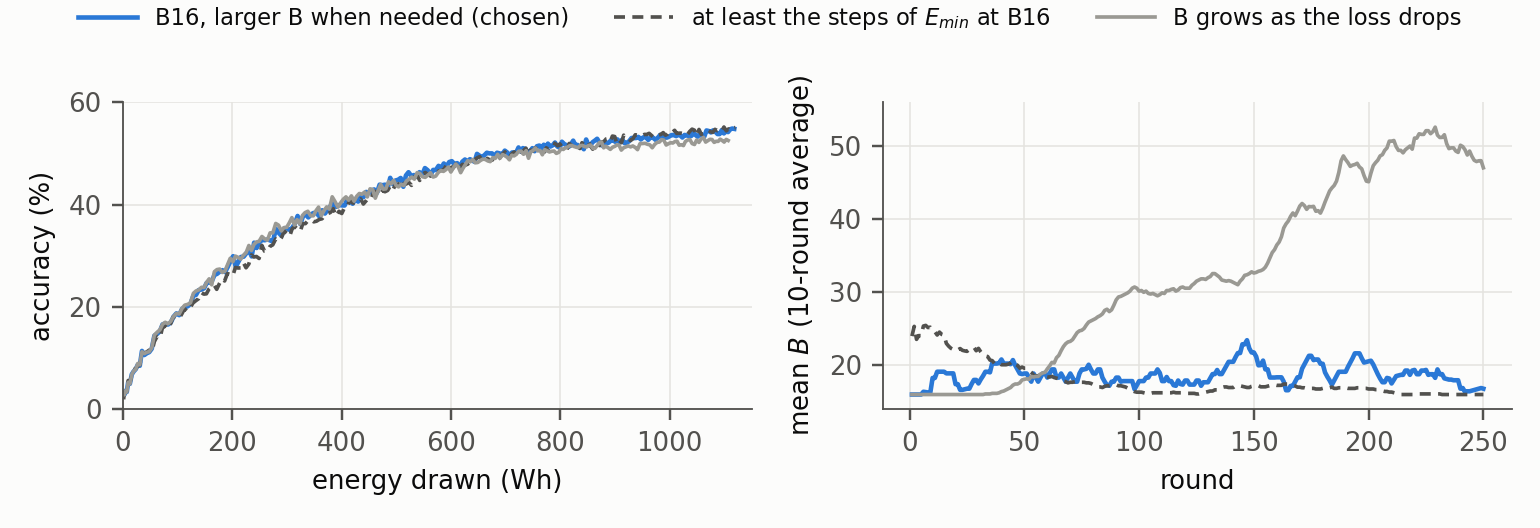
\includegraphics[width=0.8\textwidth]{report17_figs/fig_batch_rules_seed7.png}
  \caption{Batch rules on seed 7: accuracy against energy (left) and mean $B$
  of the trained clients (right).}
  \label{fig:rules}
\end{figure}

We keep the first rule: the client starts from $B = 16$, lowers $E$ if needed,
and moves to a larger $B$ only when not even $E_{\min} = 2$ epochs fit at $B =
16$ within the deadline or the battery. It is the best or tied on every metric,
and with the new cost of the batch it is no longer fixed: $B > 16$ appears in
130 of 250 rounds (18 before). $B$ adapts to the constraint of the device, not
to the progress of training; the rule that follows the loss moves $B$ the most
(16 to 50) but loses 2 points at the end because it does fewer steps.

%======================================================================
\section{Final campaign: first results}
\label{sec:final}

Everything is rerun with the new physics in one folder (135 runs, about 7
days): SAGE-smart with the three batteries (27), the mismatch (9: the server
predicts the SoC with the linear battery, the phones are Datasheet and predict
their own consumption with the true battery, no noise on the charge indicator),
FedAvg at $B = 16$ with and without guard (18), FedAvg at $B = 128$ with
learning rate 0.01/0.04/0.08 (27), FedProx, SAGE and ESCS at $B = 16$ (54). For
today we ran only seed 2026 with the Datasheet battery: 11 of 15 runs are done;
the mismatch at $\beta = 0.5$ produced no results and is being checked, and at $\beta = 1.0$
SAGE-smart, FedAvg $B = 16$ and ESCS-MD are still missing.

\begin{table}[H]
  \centering\small
  \caption{Seed 2026, Datasheet battery, 250 rounds.}
  \label{tab:final}
  \begin{tabular}{llcccccc}
    \toprule
    $\beta$ & Algorithm & Acc. (\%) & Energy (Wh) & Time (h) & Depleted & Wh to 40\,\% & Acc. at 600 Wh \\
    \midrule
    \multirow{5}{*}{0.1}
      & SAGE-smart          & 52.0 & 1117 & 9.0  & 3  & 502 & 42.4 \\
      & SAGE-smart mismatch & 50.4 & 1102 & 9.0  & 4  & 509 & 42.2 \\
      & FedAvg $B = 16$     & 55.0 & 2079 & 29.6 & 72 & 541 & 40.7 \\
      & FedAvg guard        & 56.4 & 2306 & 30.9 & 44 & 575 & 41.0 \\
      & ESCS-MD $B = 16$    & 53.9 & 2093 & 26.6 & 32 & 594 & 40.4 \\
    \midrule
    \multirow{4}{*}{0.5}
      & SAGE-smart          & 57.7 & 1086 & 8.9  & 3  & 273 & 52.5 \\
      & FedAvg $B = 16$     & 58.5 & 2116 & 27.2 & 65 & 395 & 46.3 \\
      & FedAvg guard        & 59.2 & 2273 & 27.9 & 41 & 376 & 47.6 \\
      & ESCS-MD $B = 16$    & 56.4 & 2111 & 27.3 & 35 & 433 & 45.0 \\
    \midrule
    \multirow{2}{*}{1.0}
      & SAGE-smart mismatch & 58.4 & 1085 & 8.7  & 3  & 235 & 53.8 \\
      & FedAvg guard        & 59.6 & 2223 & 26.5 & 37 & 351 & 48.4 \\
    \bottomrule
  \end{tabular}
\end{table}

\begin{figure}[H]
  \centering
  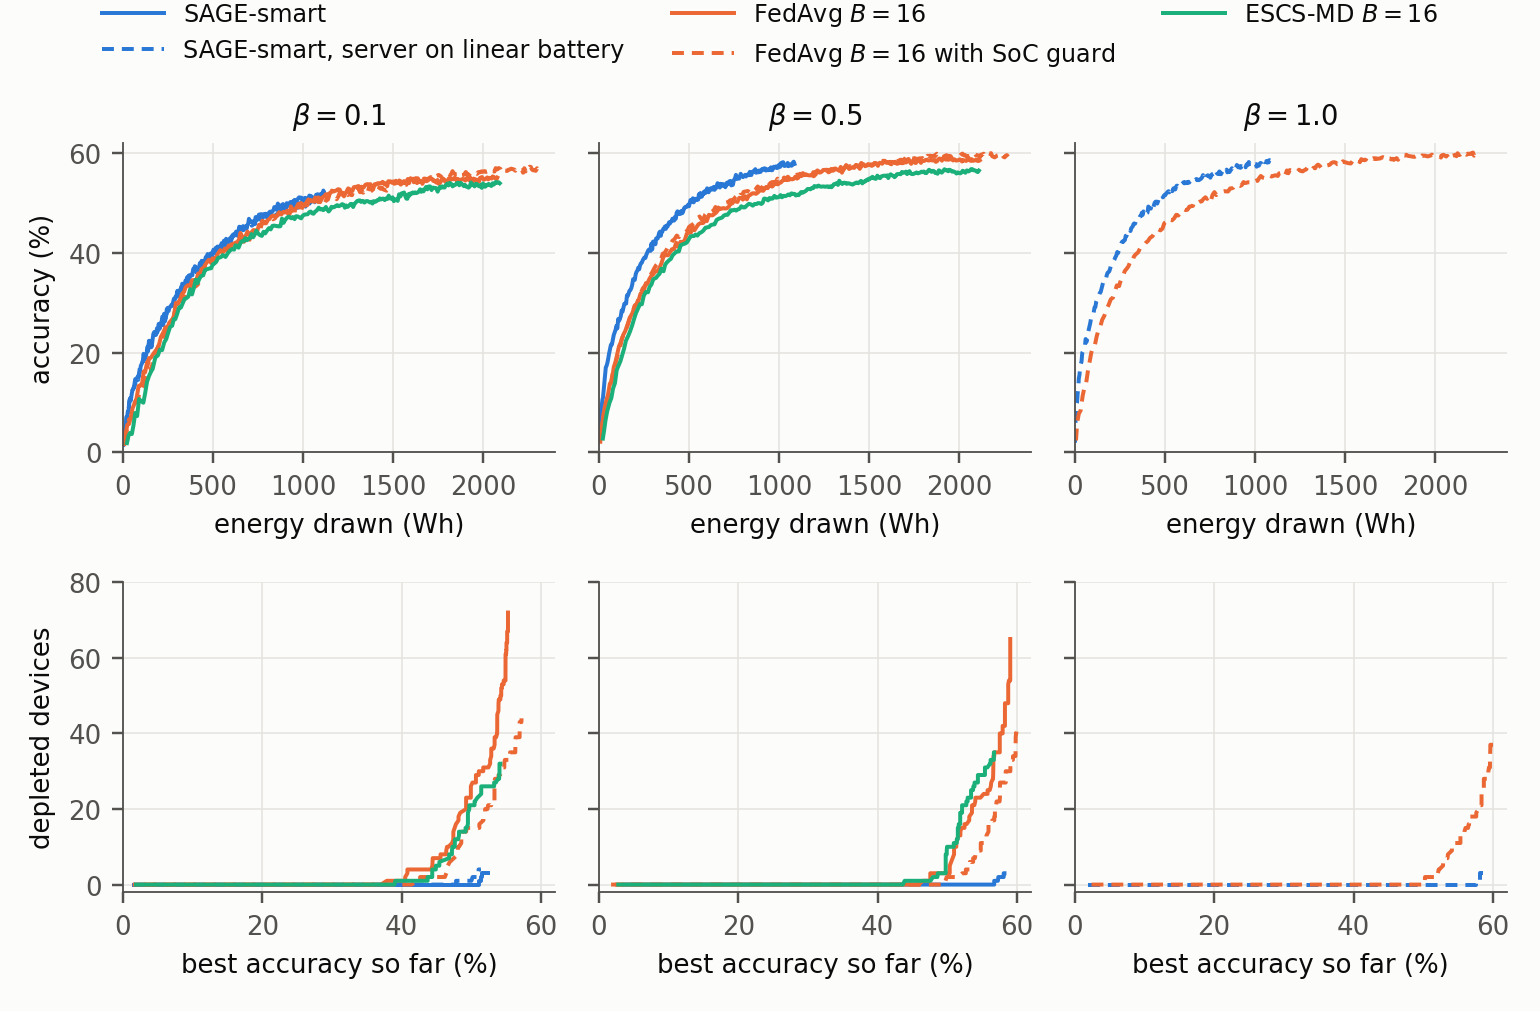
\includegraphics[width=0.88\textwidth]{report17_figs/fig_final_seed2026.png}
  \caption{Seed 2026, Datasheet battery. Top: accuracy against the energy drawn
  from the batteries. Bottom: depleted devices against the best accuracy
  reached so far. At $\beta = 1.0$ only the runs already finished.}
  \label{fig:final}
\end{figure}

\begin{itemize}
  \item At the same energy SAGE-smart is ahead at every $\beta$. To reach
        40\,\% it needs 7\,\% less energy than FedAvg at $\beta = 0.1$, 27\,\%
        less than the guard at $\beta = 0.5$ and about 33\,\% less at $\beta =
        1.0$, in line with the 23\,\% of the validations.
  \item At $\beta = 0.1$ the gap at the same energy is only 1--2 points, within
        the noise of a single seed: this is the weak point.
  \item After 250 rounds the baselines are 1--4 points higher, but they draw
        twice the energy and take three times the simulated time; after 9 h
        SAGE-smart is 4.5--6 points ahead.
  \item SAGE-smart depletes 3 devices, the baselines 32--72. The guard lowers
        FedAvg from 72 to 44 and from 65 to 41 for +0.7--1.4 points and
        7--11\,\% more energy: phones still die from background use.
  \item The mismatch costs 1.6 points at $\beta = 0.1$ with the same energy and
        depleted devices: the client checks its true battery before training,
        so the error of the server matters little.
  \item ESCS-MD at $B = 16$ stays below FedAvg at $B = 16$.
\end{itemize}

%======================================================================
\section{Next}
\label{sec:next}

\begin{itemize}
  \item Finish the final campaign (about 6 more days) and find out why the
        mismatch run at $\beta = 0.5$ produced no results.
  \item Decide whether SAGE and ESCS at $B = 16$ are needed also with the Ideal
        and Peukert batteries (90 runs, about 6 days).
  \item With all seeds, check whether the small gap at $\beta = 0.1$ holds.
\end{itemize}

\end{document}
